\section{研究背景及动机}
\label{chap:linphone:motivation}

本章主要介绍Linphone的基本特性,对应的平台为Android端,采用的Linphone Android端版本为4.2.3,Linphone SDK版本为4.3.0。

\subsection{Linphone软件架构}
\label{chap:linphone:motivation:struct}

\insertFigure{
	\begin{figure}[htbp]
		\centering
        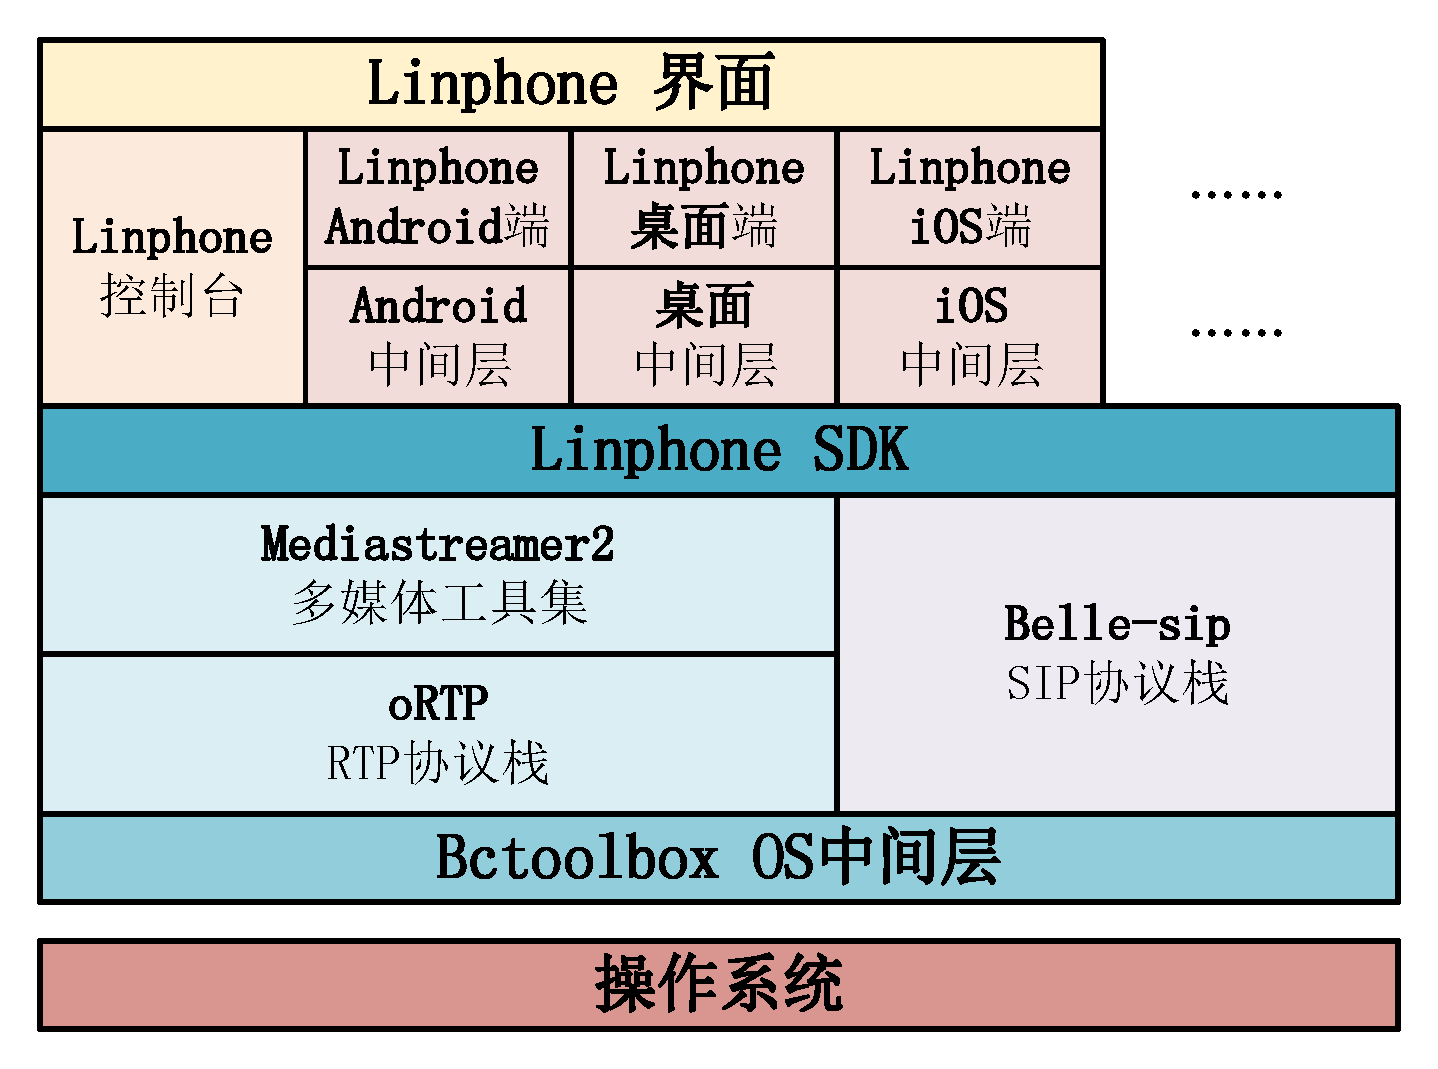
\includegraphics[width=0.65\textwidth]{chapters/chapter6/figures/linphone-struct.pdf}
        \caption{Linphone软件架构图}
        \label{fig:6:linphone-struct}
    \end{figure}
}

如图\ \nref{fig:6:linphone-struct},完整的Linphone应用包括Linphone SDK及Linphone 界面两部分组成。其中Linphone SDK具备跨平台特性,为界面提供传输控制接口,内部封装了SIP及RTP相关的网络协议栈、传输控制、编解码器以及控制工具。Linphone界面面向不同的设备环境,基于Linphone SDK提供用户交互接口。

Linphone SDK中,主要包括基于RTP的Mediastreamer2工具集,以及基于SIP的Belle-sip协议栈。根据数据类型的划分,Linphone中的控制消息及用户聊天信息均通过SIP进行传输,而语音及视频数据通过RTP进行传输。因此,音视频数据流在Mediastreamer2中经过编码器处理后,转换为RTP数据包经oRTP协议栈进行传输。基于主动丢包的时间隐通道,需要在oRTP中控制数据包传输调度,从而确保丢弃的数据包序号与接收方的观测值一致。

对用户友好的时间隐通道,通常也应具备UI层用户接口,通过UI接口进行隐蔽消息设定、隐蔽消息提取,以及查看当前时间隐通道的传输状态。Linphone环境下实现该功能,不仅需要在Linphone SDK中添加数据包控制模块,还需要在SDK中添加额外的控制端口。

\subsection{Linphone音视频编码方案}
\label{chap:linphone:motivation:coding}

\insertTable{
	\begin{table}[htbp]
      \centering
      \caption{Linphone及VoLTE的音视频编码方式}
      \label{tab:6:motivation:coding}
          \begin{tabular*}{0.9\textwidth}{@{\extracolsep{\fill}}cccc}
            \toprule
            应用环境 & 数据对象 & 可选编码 & 默认编码 \\
            \midrule
            \multirow{2}{*}{VoLTE}
            & 音频 & AMR-WB, AMR & AMR-WB \\
            & 视频 & H.264 & H.264 \\
            \\
            \multirow{4}{*}{Linphone\ (v4.2.3)}
            & \multirow{3}{*}{音频} & opus, speex, g711, g729, & \\
            & & gsm, iLBC, AMR, AMR-WB, & opus \\
            & & g722, SILK, iSAC, BV16 & \\
            & 视频 & VP8, H.264, H.265 & VP8 \\
            \bottomrule
          \end{tabular*}
    \end{table}
}

在音视频编码方面,VoLTE与Linphone存在区别。Linphone作为开源的VoIP应用,支持了主流的音视频编码方法,从而适应不同应用环境之间的编解码方案。而VoLTE无需支持复杂的应用环境,通话采用的编码方式及码率相对稳定。表\ \nref{tab:6:motivation:coding}对比了Linphone及VoLTE支持的编码类型,其中,VoLTE通常采用AMR-WB+H.264的组合方式\nupcite{8288828, ZHANG201929},而Linphone通常采用opus+VP8的组合方式。

对于语音信道来说,Linphone与VoLTE在数据包发送速率方面一致。VoLTE采用AMR-WB编码,在非静音期每{20\ ms}发送一个数据包,平均数据包发送速率为{50\ pkts/s};Linphone采用opus编码,采样频率为{48\ kHz},平均每{20\ ms}发送一个数据包,平均数据包发送速率为{50\ pkts/s}。

对基于主动丢包的时间隐通道来说,宿主信道的数据包发送速率越高,时间隐通道能够达到的传输性能越高。对于本文中提出的时间隐通道构建方法,鲁棒性测试等已经通过模拟实验验证,只需要验证主动丢包的调制方式是否有效。因此,Linphone环境中选择语音信道进行测试,虽然传输性能受影响,但验证结论仍然有效。

\subsection{Linphone网络传输模式}
\label{chap:linphone:motivation:net}

基于Linphone的VoIP通话,需要面临复杂的用户接入网络。在当前IPv4网络环境中,用户设备所获取的IP通常经过了NAT(Network Address Translation)转换,因此无法直接建立P2P(Peer to Peer)会话。为解决该问题,常用的方法包括基于隧道的P2P链接,以及基于公网服务器的数据转发。对于VoIP应用来说,通过中间服务器进行转发,产生的传输延迟不可忽略,影响用户体验。因此,Linphone支持STUN(Session Traversal Utilities for NAT)及TURN(Traversal Using Relay NAT)创建端到端链接,并且支持自定义隧道服务器进行数据转发\nupcite{5673073}。

Linphone与VoLTE在网络传输机制方面,存在固有差异。Linphone为建立端到端链接,需要与公网服务器进行交互,从而确定客户端在公网中对应的IP地址及端口。然而在实际测试中,Linphone创建P2P链接的成功率较低,常见的NAT场景中成功率不超过30\%,并且在更加复杂的网络环境中难以运作\nupcite{5673073}。而VoLTE是运营商通信业务的一部分,直接接入运营商网络,并且当前VoLTE多运行在IPv6网络中,具备直接点对点传输能力,无需考虑NAT环境。

对于VoIP等高实时性应用来说,网络延迟影响通话质量\nupcite{8698715}。即使在编码方面进行了优化,网络对通话质量的影响仍然是决定性因素\nupcite{7478066,8698715}。根据本文\ \nref{chap:linphone:motivation:coding}中对编码方式的分析,Linphone视频数据流具有较高的数据包发送速率,在创建P2P链接失败的情况下,无法有效保证视频通话的流畅性和实时性。因此,基于Linphone的时间隐通道原型系统,选择Linphone语音流作为传输载体,并在不同的网络环境中进行测试。

\subsection{研究动机}
\label{chap:linphone:motivation:sum}

\insertFigure{
	\begin{figure}
		\centering
        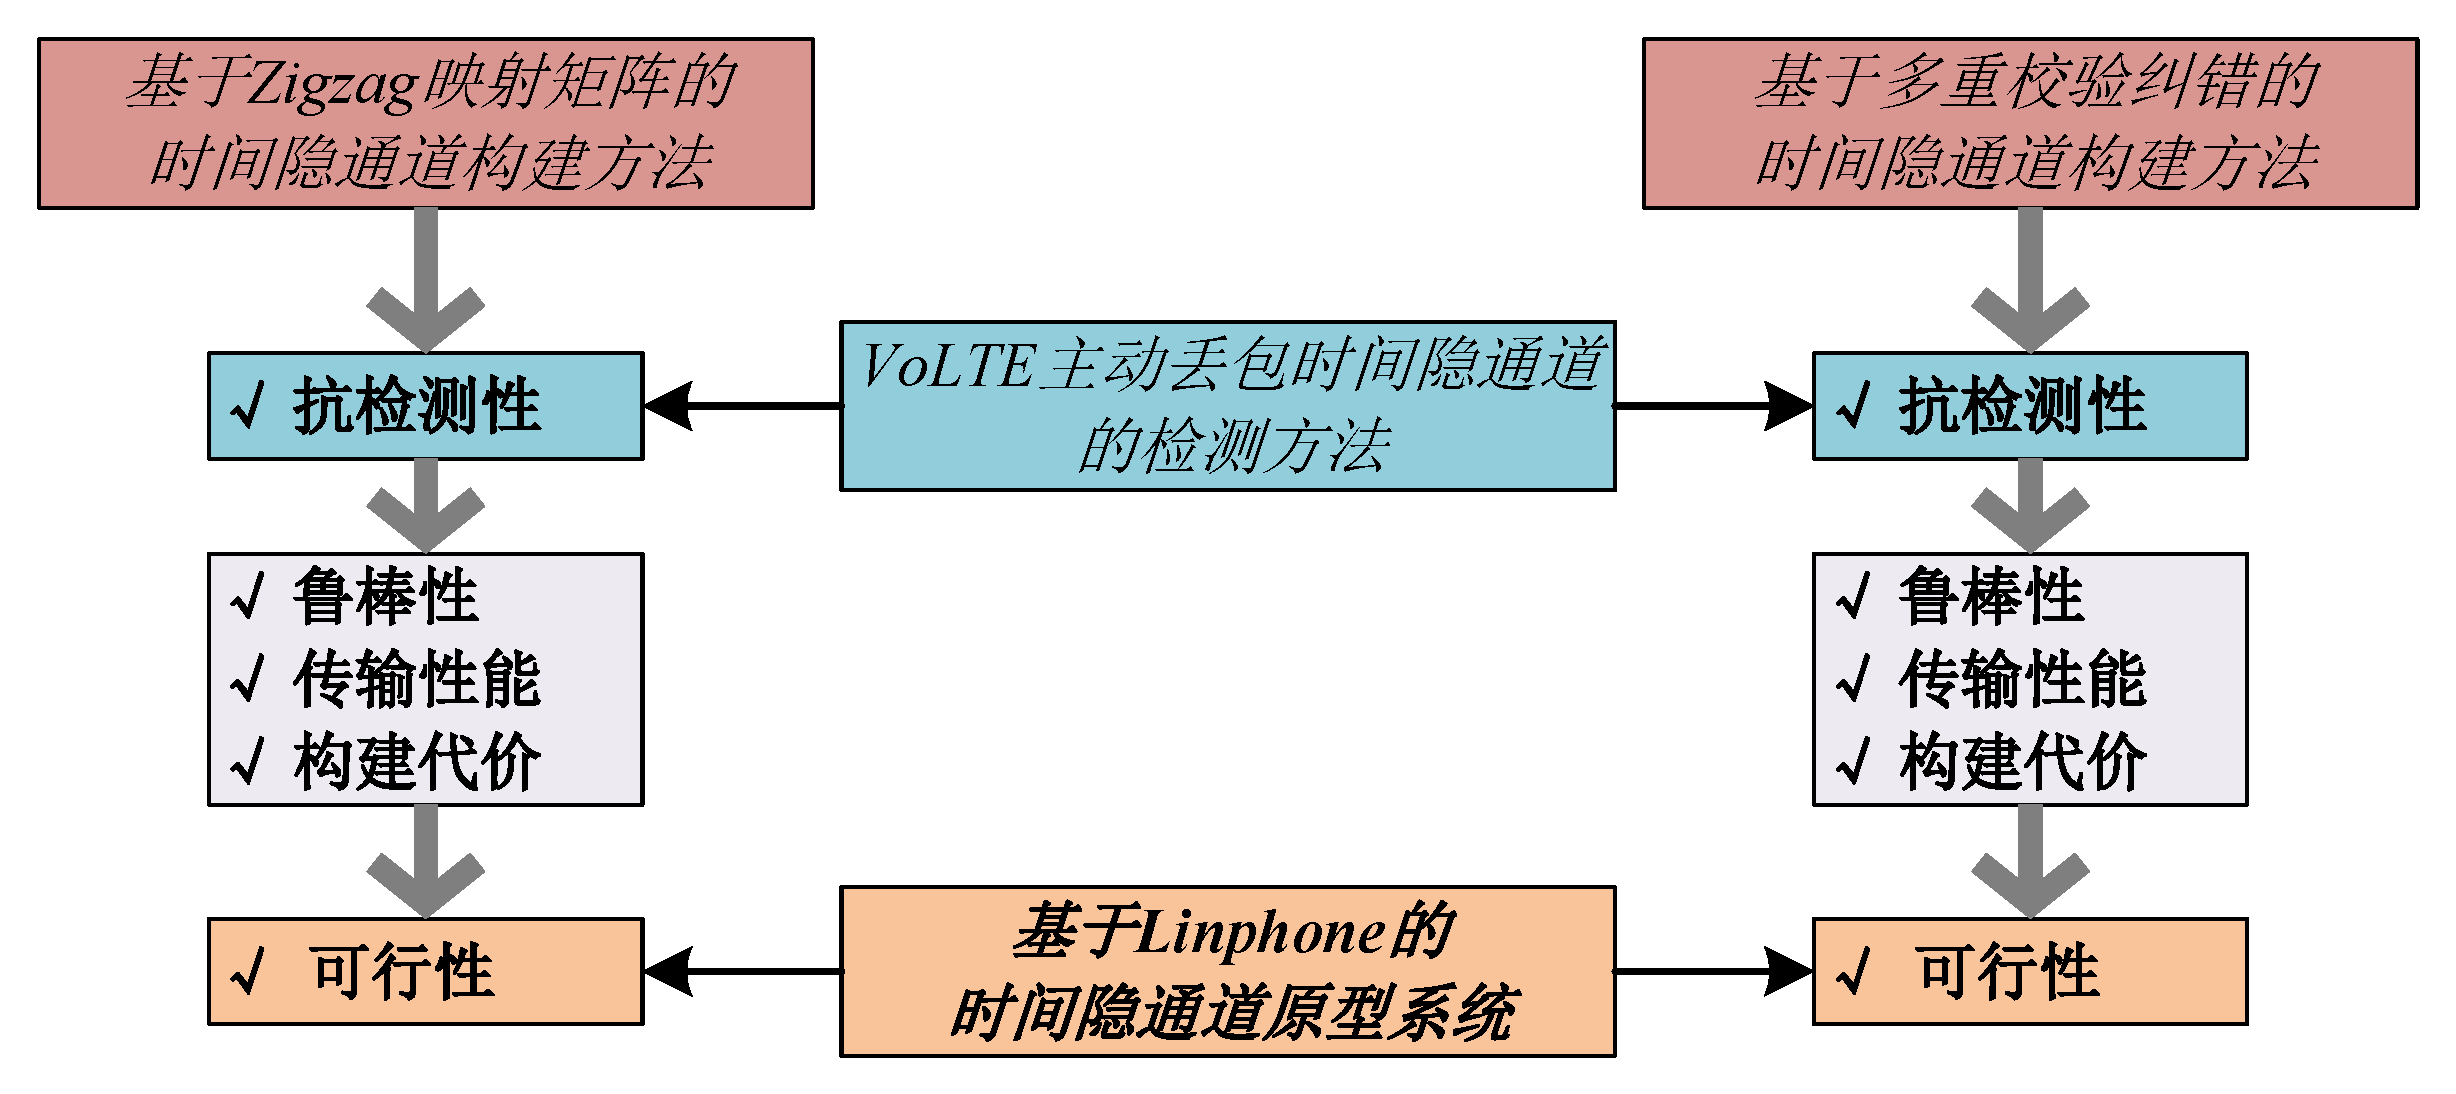
\includegraphics[width=0.9\textwidth]{chapters/chapter6/figures/chapter-relationship.pdf}
        \caption{基于Linphone的时间隐通道原型系统关联图}
        \label{fig:6:chapter-relationship}
    \end{figure}
}

借助Linphone平台构建时间隐通道原型系统,利用了Linphone与VoLTE在传输模式上的相似性,从而验证基于主动丢包构建时间隐通道的模式。如图\ \nref{fig:6:chapter-relationship},在本文\ \nref{chap:zigzag:results}及本文\ \nref{chap:hash:result}中,通过数据模拟的方式,对两种时间隐通道的抗检测能力、鲁棒性、构建代价及传输性能进行了评估。因此,基于Linphone的时间隐通道原型系统,以实验证明其可用性及有效性,从而证明主动丢包在原理及应用方面切实有效。